\documentclass[runningheads,a4paper]{llncs}
% proper encoding
\usepackage[T1]{fontenc}

% autoref command
\usepackage[pdftex,urlcolor=black,colorlinks=true,linkcolor=black,citecolor=black]{hyperref}

% better typography
\usepackage[activate=compatibility]{microtype}

% graphics
\usepackage{graphicx}

\usepackage[lofdepth,lotdepth]{subfig}

% URLs
\usepackage{url}

\begin{document}

\mainmatter

\title{Enriching Content Objects for Multimodal Search with Data from the Linking Open Data Cloud}
\authorrunning{Enriching Content Objects for Multimodal Search with LOD Cloud Data}

\author{Jonas Etzold\inst{1} \and Thomas Steiner\inst{2} \and Arnaud Brousseau\inst{2}\thanks{The author was an intern at Google Germany GmbH at time of core development.} \and Paul Grimm\inst{1}}

\institute{\label{fulda}Hochschule Fulda, Marquardstr. 35, 36039 Fulda, Germany\\
\urldef{\emails}\path|{jonas.etzold,paul.grimm}@hs-fulda.de|\emails\\
\and Google Germany GmbH, ABC-Str. 19, 20355 Hamburg, Germany\\
\urldef{\emails}\path|{tomac,arnaudb}@google.com|\emails\\
}

\maketitle

\setcounter{footnote}{0}

\begin{abstract}
In this paper, we report on the \mbox{I-SEARCH} EU (FP7 ICT STREP) project
whose objective is the development of a~multimodal search engine that supports multimodal
in- and output, as well as multimodal query refinement.
An important aspect of \mbox{I-SEARCH} is the so-called
\emph{Rich Unified Content Description} \emph{\mbox{(RUCoD)}} format
for the description of low and high level features of content objects---rich
media presentations, enclosing different types of media.
We have developed a~tool called \mbox{\emph{CoFetch}}
for the creation of such content objects,
which partly retrieves its data from the Linking Open Data cloud.
During the session, we will present a~live demonstration of the \mbox{I-SEARCH}
search engine and \mbox{\emph{CoFetch}}, and---via pre-defined use cases---show
how we imagine multimodal search in the future.
We are looking for networking opportunities with projects dealing with
semantic annotation of multimedia archives and 
projects interested in \emph{RUCoD} feature extraction techniques.
\end{abstract}

\section{Introduction}
Search engines over the years have coined a~common interaction pattern:
the search box.
We enhance this interaction pattern with context-aware modality input toggles
that create modality query tokens in the \mbox{I-SEARCH} search
box\footnote{See \url{http://isearch.ai.fh-erfurt.de/} for a~live demonstration.}.
The concept-centered \mbox{I-SEARCH} search engine lets users search
by using different modalities and combinations of modalities.
Supported modalities are \emph{audio}, \emph{video},
\emph{rhythm}, \emph{image}, \emph{3D object}, \emph{sketch}, \emph{emotion},
\emph{social signals}, \emph{geolocation}, and \emph{text}.
For example, in order to get a~holistic view of the concept of
Leonardo da Vinci's painting of \emph{La Joconde},
a~user could search via a~photograph of the painting,
and---besides the textual description---also get back
the exact geolocation of the painting in the Louvre museum,
a~video of a~relevant section of a~Louvre tour,
or an audio recording of an explanation of the painting by a~museum guide.

\section{Rich Unified Content Description (\emph{RUCoD})}
In order to allow for the before-mentioned concept-centeredness of
\mbox{I-SEARCH}, in the context of the project we have first introduced
the notion of so-called \emph{content objects}, and second,
a~description format named \emph{Rich Unified Content Description
\mbox{(RUCoD)}}~\cite{ijmis2010}.
Content objects are rich media presentations, enclosing different types of media,
along with real-world information and user-related information.
\mbox{\emph{RUCoD}} provides a~uniform descriptor for all types of content objects,
irrespective of the underlying media and accompanying information.
In the next section, we will introduce a~tool for the creation of such content objects.

\section{\mbox{\emph{CoFetch}}---A~Tool for the Creation of Content Objects}
\mbox{\emph{CoFetch}} is a~content object creation tool
that can be operated in a~fully automatic, or in a~semi-supervised way.
In order to generate content objects for a~given term- and category-based query,
it harvests textual and image data from DBpedia
via the DBpedia Lookup service~\cite{lookup},
3D models from Google 3D Warehouse~\cite{3dwarehouse},
images from Flickr~\cite{flickr}, videos from YouTube~\cite{youtube},
audios from Freesound~\cite{freesound},
and historical weather data from Weather Underground~\cite{wunderground}.
In order to decide on the most relevant results from each service,
a~Levenshtein distance function based on the titles and descriptions is used.
First, we generate a~list of occurrences of the query terms
within the results' textual data.
Second, we generate a~list of distances between query and result titles.
Third, the end result with the two most relevant items is determined.
Finally, a~descriptor file with extracted \emph{\mbox{RUCoD}} features
and pointers to all media items is generated.

\begin{figure}[]
\vspace{-1.0em}
  \centering
    \subfloat[][Architecture of the \mbox{\emph{CoFetch}} tool.]{
      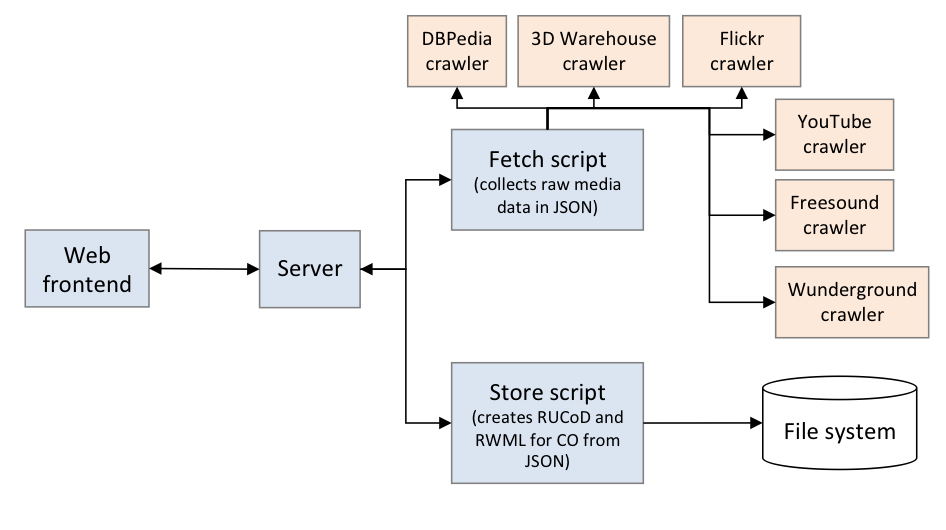
\includegraphics[width=0.54\textwidth]{architecture.png}
      \label{fig:architecture}}
    \qquad
    \subfloat[][The \mbox{\emph{CoFetch}} tool's GUI.]{
      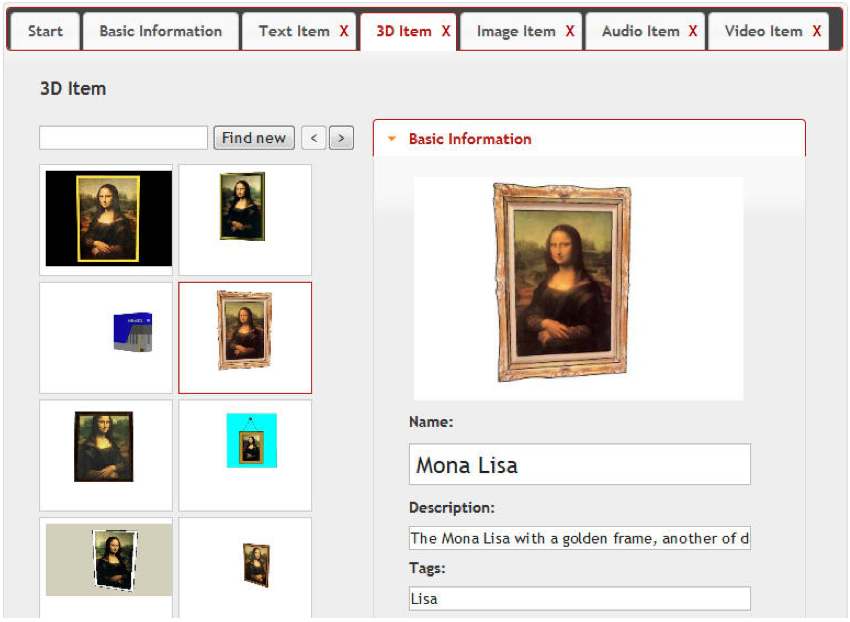
\includegraphics[width=0.35\textwidth]{screenshot.png}
      \label{fig:screenshot}}
\caption{The \mbox{\emph{CoFetch}} tool uses among others data from the Linking Open Data cloud (\url{http://lod-cloud.net/}) for the generation of content objects.}
\label{fig:cofetch}
\vspace{-2.8em}
\end{figure}

\bibliographystyle{splncs03}
\bibliography{eswc2012}

\end{document}